\documentclass[a4paper]{report}

\usepackage[utf8]{inputenc}
\usepackage[swedish]{babel}
%\usepackage{hyperref}
\usepackage{graphicx}
%\usepackage{csquotes}

\title{Individuell reflektionsrapport: förstudie, grupp 5}
\author{Max Danielsson}
\date{20 November 2013}
\begin{document}
   \maketitle

\section*{Introduktion}

Denna rapport är en respons på de följande frågorna. Frågorna har besvarats
kategoriskt i samma följdordning som frågorna är ställda.

\begin{quote}
    \begin{itemize}

        \item Vad ser ni som mest viktigt att få till i början av ert projekt och hur kommer
                ni  använda er av detta?
        \item Hur har ni satt ihop er grupp?
        \item På vilket sett kommer er grupp att vara effektiv?
        \item Hur har ni kommit fram till de mål ni har med ert projekt?
        \item Hur kommer ni att kunna säga i slutet om ni uppnått era mål?
        \item Hur kommer ni se till att ert projekt håller en kvalitet som behövs för
                marknaden?
    \end{itemize}
\end{quote}

\section*{ Projektplanering }

Vad vi känner är viktigast är att först fastställa spelets designmål och vad
spelet behöver tekniskt för att realiseras. För detta så skriver vi ett
speldesignsdokument som definierar spelet som det är tänkt att vara. Vissa
aspekter av spelet som vi sedan tidigt inser är kärnan till spelupplevelsen och
det mest tekniskt utmanande eller tekniskt okänt är det som kräver störst
kunskap om hur det kan implementeras. Sedan så skriver vi tekniska rapporter
på de aspekter som vi känner kräver en förstudie för att lättare få en känsla
av hur stor eller utmanande en viss feature kan tänkas vara. Rapporten försöker
utforska hur problemet bäst löses och ger en kort sammanfattning med ett
förslag på hur problemet bör tacklas inom projektets ramar och vad det kan
innebära samt möjliga fallbacks om lösningen visar sig att vara för svår eller
omöjlig.
 
Med vissa gameplay features så räcker inte en rapport utan de vill helst
prototypas för att få en idé om spelet kommer att realiseras på det sätt vi
tänker oss och snabbt se om det är "roligt". Det kan vara en bra metod för att
snabbt avverka vissa idéer innan vi ens har påbörjat utvecklingen av spelmotorn
vilket i bästa fall resulterar i att utvecklingsplanen får en bättre
startriktning. Detta är viktigt då spelmotorn väntas vara den mest tidskrävande
aspekten av utvecklingsfasen.

Denna tidigare nämnda dokumentation kommer förhoppningsvis att underlätta
planering och synkronisering i arbetet, både arkitekturellt och tidsmässigt.
Det kommer även ha klarlagt för alla medlemmar vad som förväntas byggas och
ungefär hur det kommer se ut i slutändan för att underlätta sammansättning av
resultat samt användning av olika moduler i systemet.

Genom projektets gång så kommer vi använda oss av scrum som vi kombinerat med
kanban där vi taget flödet från kanban och infört det i barbetningen av tasks
för att skapa en struktur på arbetet. Från programmerarens perspektiv så är
flödet för tillfället indelat i tre steg, Design, Test Development och
Development.  Alla medlemmar är sedan tidigare ovana vid att följa TDD
tankegången vilket är anledningen till att de två första stegen är explicita i
flödet. Tanken med Design och Test Development -stegen är för att lite smått
tvinga in ett nytt tankesätt baserat på TDD. Vi skall försöka ha en tydlig plan
och någon sånär färdiga tester innan vi faktiskt börjar utveckla något, mest
för att hålla kvalitén på projektet högt när vi närmar oss de senare
utvecklingsstadierna Detta tros behövas då vi aldrig tidigare jobbat i ett
projekt av denna skala och tidslängd och vi har sedan tidigare erfarit att kod
snabbt ruttnar om man inte aktivt motarbetar det, redan under ganska korta
tidperioder.

Det finns även en speciell pipeline for content generering där stegen är lite
mer flertaliga och uppdelade i de olika faserna som Art Lead med resten av TA
gruppen anser är vettiga för konstruktion av saker som modeller, animationer,
texturer, etc.

\section*{Gruppuppsättning}

Tidigt så lade vi ett värde på att införa roller i projektet, mest för att
fastställa så att det finns någon ansvarig i de olika aspekterna av projektet, men
även för att kunna underlätta arbetsflödet genom att garantera att visa
personer har viss temaspecifik fokus under projektets gång. Projektet
anses vara för stort för att en individ skall kunna hålla kolla på helheten,
även om det bara handlar om en medeldjup nivå.

De roller vi infört är följande.

\textbf{Projektledare} (Alexander Vestman): Ansvarig för projektet som helhet, han agerar lite som en
producent i det att han ser till så att projektet är realistiskt, ifrågasätter
allt för ambitiösa idéer, försöker hålla kvalitén hög som produkt. Han försöker
även se till att milstolpar och deadlines möts, följer upp på planer som skall
genomföras och har en ytlig helhetsbild av hela projektet.

\textbf{Game Designer} (Tim Henriksson): Ansvarig för att dokumentera speldesignen, skall hålla i och
förespråka spelet vision så att alla medlemmarna jobbar mot samma mål. Skall ha
en god översikt på hur spelet skall fungera och kännas när det spelas.

\textbf{Lead Artist} (Lukas Orsvärn): Ansvarar för all produktion av art, dvs modeller, animation,
texturer, koncept-art och dylikt. Ser till så att alla artister håller en
homogen stil och hög kvalitetsnivå. Håller i alla tidsplaneringsmöten för art.
Har mandat att säga sista ordet i ett beslut angående art utseende och känsla.

\textbf{Lead Programmer} (Max Danielsson): Ansvarar för all produktion och kvalitet av
mjukvara och teknik, dvs programkod, script, arkitekturell design, användning
av tekniker och bibliotek.  Håller i tidplaneringar för all programmering. Har
mandat att säga sista ordet i beslut angående tekniska lösningar och val.
Ansvarar för att tillräcklig dokumentation av systemet finns för att möjliggöra
effektivt arbete.

Övriga medlemmar har ingen explicit roll mer än medarbetare. Våra roller inte
inte tänkta att vara heltidsjobb, men vi inser att de kommer ta en del tid från
andra ansvar vilket vi måste bearbeta då det är tänkt från kursens perspektiv
att alla medlemmar skall vara lika mycket aktiva i den faktiska utvecklingen
(programmering etc.)

\section*{Effektivitet}

Det finns stora förhoppningar om att våra roller samt förplaneringen av
projektet med dokumentation av lagom grad samt scrummetoden med tasks placerade
på domänspecifika individer skall tillåta oss att lättare kunna fokusera på
vårt specifika arbete. Jag har av egen anekdotisk erfarenhet kommit fram till
att projekt av sin natur har väldigt många frågor som måste ges svar på, frågor
som kanske bör ställas till övriga medlemmar och påverkar deras arbetsflöde,
många gånger så riskerar svaret eller lösningen på en sådan fråga i att
projektet bryter av huvudspåret om individen inte har samma helhetsbild av
projektet som resten av gruppen. Därför är förplanering och diskussioner om
viktiga, det ger en delad vision som minimerar antalet frågor under
utvecklingens gång. Hur saker och ting faktiskt kommer att lösas i detalj är
däremot svårt att svara på i förväg och det finns inga förhoppningar om att
planering på den nivån kommer att ge något om den utförs för långt i förväg.

\section*{ Projektmål }

Vi har ambitionen att vårt spel skall vara tillräckligt, unikt, roligt och
intressant för att potentiellt bli nominerade till Swedish Game Awards. Vi har
även försökt ta hänsyn till gruppen uppbyggnad för att arbeta på en spelidé som
matchar våra förkunskaper samt tillåter oss som individer att utvecklas genom
att testa nya tekniker och lösningar utan att det hotar spelets kärna.

Med dessa aspekter i åtanke så konstruerade vi en spelidé som har en liten
enkel kärna som vi prioriterar som viktigast i projektet. Denna kärna har vi
redan nu prototypat i viss mån för att få en så tydlig bild som möjligt av hur
kärnan kan upplevas och fungera i slutprodukten.
Utöver den centrala biten så har vi andra övriga features som utökar spelets
kvalitet men som kan tas bort om de inte anses möjliga eller tidseffektiva,
eller rent av inte är tillräckligt tekniskt utmanande för kursen krav.


\begin{figure}[h!]
  \caption{ Grova projektmilstolpar }
  \centering
    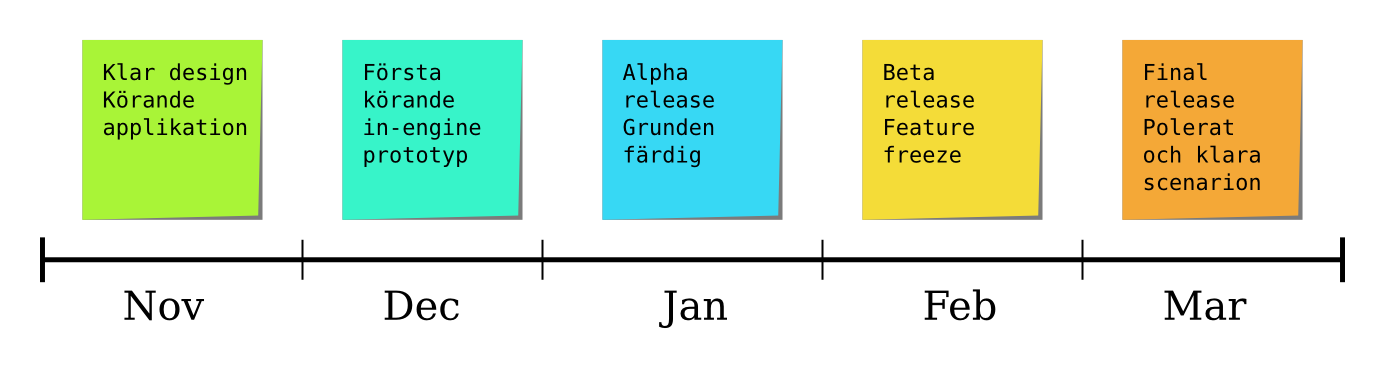
\includegraphics[width=1.0\textwidth]{Milstolpar_large.png}
\end{figure}


\section*{ Projektmålskriterier }

Det finns inte för tillfället några starka kriterier för vad som definierar att
projektet är färdig. Det finns en lös vision som sannolikt kommer att mogna och
utvecklas under projektets gång. På en bredare basis så är projektens utgångsmål
uppnådda om spelet har en sådan kvalitet och spelbarhet att det går att direkt
jämföra med tidigare års kandidater till Swedish Game Awards, men denna
jämförelse kan vara förrädisk och svår att genomföra.

Mer exakta projektmål kan komma att etableras som faktiskt specificerar vad som
krävs för att just denna spelidé och detta projekt uppnår en nivå som är
färdig. Det är direkt användbart om man vill ha ett väldigt tydligt slutmål när
projektplaneringen genomförs i lite större detalj.

\section*{ Projektkvalitetsmål }

Tanken är att de fyra roller skall tillsammans försöka se till så att hela
projektet uppnår en kvalité som hela gruppen samt kursexaminatorer är nöjda
med. Genom att ge var roll ett specifikt domänområde så kan de individerna
fokusera på att finna sätt att se till så kvalitén är hög inom just deras domän
och kan således gå betydligt djupare, det ger även en fin naturlig konflikt
mellan rollerna där de alla tydligt uttrycker sin egna domäns kvalitetskrav
vilket förhoppningsvis gör diskussionerna lite mer färgade.

En stor del av att se till så en viss kvalité uppnås är genom att vi först
försöker inse vad kvalité innebär för vår domän. Mycket handlar om att ytligt
jämföra produkten med andra liknande produkter på marknaden för att se om det
finns något marknadspotential. Syftet med att ha Swedish Game Awards som mål
för projektet bemöter detta kvalitets krav genom att tvinga oss till att
försöka uppnå ett relativt tydligt mål och specifikt ideal inom en viss domän
istället för något bredare som kan vara svårare att definiera.

Min specifika roll som är teknisk handlar om att försöka uppnå en kvalitet av
verktygen och de tekniska arbetsmiljöerna som möjliggör att medarbetare
underlättas i sitt arbete för att uppnå denna marknadsstandard.
\end{document}
